\documentclass[12pt,letterpaper]{article}

\PassOptionsToPackage{hyphens}{url}
\usepackage[pdftex, bookmarksopen=true, bookmarksnumbered=true,
pdfstartview=FitH, breaklinks=true, urlbordercolor={0 1 0}, citebordercolor={0 0 1}]{hyperref}

% === MARGINS ===
\addtolength{\hoffset}{-0.75in} \addtolength{\voffset}{-1.25in}
\addtolength{\textwidth}{1.5in} \addtolength{\textheight}{2.25in}

% == ENVS ==
\newenvironment{tightcenter}{%
  \setlength\topsep{0pt}
  \setlength\parskip{0pt}
  \begin{center}
}{
  \end{center}
}

% == PACKS ==
\usepackage{color,soul}
\usepackage{graphicx}
\usepackage{calc} % To scale \pagewidth with \real{float}
\usepackage{pgfplots} % To draw histogram
\pgfplotsset{compat=1.17} % request specific version of pgfplots
\usepackage{calc} % to use \real for text -> numeric
\usepackage{pgf} % to store numeric variables
\usepackage{subcaption} % to place two figures horizontally
\usepackage{tikz}
\usetikzlibrary{automata,positioning}
\usetikzlibrary{arrows.meta, positioning, automata}
\tikzset{
  font={\fontsize{10pt}{0}\selectfont}}
\usepackage{forest}
\tikzset{
  Decision/.style = {%
    draw,
    line width=1.4pt
  },
  Lottery/.style = {%
    draw,
    line width=1.4pt
  },
  Outcome/.style = {%
    circle,
    minimum width=3pt,
    fill,
    inner sep=0pt
  }
}


  % == BIBS ==
\usepackage{natbib}
\bibliographystyle{apsr}

% == SPACES == 

% == CMMDS ==
\newcommand{\tit}{
\bf 
Mapping Regulatory Network of WTO Dispute Settlement Body Using Deep Learning
}
\newcommand\spacingset[1]{\renewcommand{\baselinestretch}
{#1}\small\normalsize}

% == VARS == 
\pgfmathsetmacro{\heatmap}{1}

% == START (PageCounter, Mode)
\begin{document}

\spacingset{1.25}

\setcounter{page}{0}
\vspace{-.1in}

% == TITLE (includes DraftDate)
{\title{
    \tit
    % \thanks{Thanks to everyone in KimResearch Group}
  }
  \author{Suyeol Yun
    % \thanks{Applicant. No Affiliates. Email: \href{mailto:syyun@snu.ac.kr}{syyun@snu.ac.kr}}}
    % \date{First Draft: October 2, 2020\\ This Draft: \today
  }
  \maketitle
}

\thispagestyle{empty}
\vspace{-.1in}

\begin{abstract}

  % Legal citation pattern in the World Trad Organization (WTO) is quite complex to understand.
  % Legal citation pattern made by the member states of the World Trade Organization (WTO) shows how members of the WTO are understanding the legal system of the WTO,
  % it is is important to recover this complex pattern efficiently. To address this issue, this paper introduces a new method
  % to map this citation pattern as a network of articles of the WTO agreement.
  % First, this paper shows why we need to use the text information in the content of the trade dispute and legal text to successfully recover the citation pattern. 
  % Then this research designs a deep neural network model to extract information inside the text content.
  % After that, we are engaging machine learning algorithm to extract the citation pattern lying in the citation pattern predicted by the neural network. By doing so, this paper introduces clusters that are found by this method that are well capturing the most important principle in the World Trade Organization.

\end{abstract}

\spacingset{1.5} % gives a slightly more margin between abstract and introduction

\section{Introduction}

The Dispute Settlement Body (DSB) of
the World Trade Organization (WTO) deals
with trade disputes between WTO members.
WTO members file a lawsuit in WTO DSB to
claim their impaired benefit related to the WTO agreements as a result of another member's possible illegal trade policy.
The judicial body of WTO DSB, \textit{Panel} or \textit{Appellate Body}, then adjudicates the dispute and submits a report in which it expresses
its judicial opinion as to whether the challenged
trade policy is inconsistent to the rules of the WTO or not \citep{world2017handbook}.


A lawsuit tends to cite multiple rules of the WTO agreement because a trade policy is usually pretty much complicated 
and one simple rule can't cover the characteristic of the trade policy at issue \citep{palmeter2004dispute}.
For example, the United States enacted \textit{Continued Dumping and Subsidy Act of 2000 (Byrd Amendment)} that distributes 
the collected anti-dumping duties to its affected domestic producers and this act was challenged with multiple rules of the WTO agreement, 
such as \textit{Anti-dumping} and \textit{Subsidy} because 
this distribution could constitute a illegal subsidy prohibited 
in the rules of the WTO agreement although it's mainly realted to the rules of the anti-dumping. 

% Todos: 
% - How to cite us laws? Byrd amendment
However, complex legal citation isn't only derived from the complicated aspect of a trade policy.
Legal citation also becomes complex because members cite the rules of the WTO strategically. For example,
members cite rules of the WTO agreement differently to limit or to encourage 
the third party participation to their lawsuit \cite{who_gets}.




% Inter-country interactions in global trade are legally regulated by the World Trade Organization (WTO).
% The members of the WTO agreed on the set of rules with the WTO agreement and sue other country's potential
% violation of the rules to the Dispute Settlement Body (DSB) of the WTO.
% When a country is suing other country to the DSB, they usually cites more than one rules of the WTO
% because a country's trade policy at issue is usually very complex thus requires many rules being combined to legallly blame the one successfully.
% For example, In the Case A, Country X cited {Articles} to blame Country Y's TRADEACTION B.

% Then why do political sceintist want to understand this complex pattern of citation? This is because of the two reasons,

% - Finding the collective understanding over the WTO's system

% - Second, upon/toward this understanding, countries design the new strategy to lead more favored result using the WTO.

% However, the methods how to deal with this complexity, has been relatively less visited by the scholars. To address this issue, I designed
% a new method that maps the countries' citation network over the WTO adjudication system. This method finds three distinctive clusters where each represents

% - market access

% - non-traiff barriers

% - regional trade agreement
% .

% This method populates a network that can showing how countries are citing which articles together in which weight to legally regulate the trade disputes inside the WTO.
% I explitly used the content of the dispute and the articles of the WTO agreement using deep neural network and machine learning algorithms.

% Moreover, to populate this network, I used 80 GATT 1994 Articles or Paragraph in the Article with 143 Trade Disputes from 1995 to 2018 where the Panel reports exists.

% Through this paper I found how wto works.
% Moreover, this complexity efficietnly caputred by this mthod could address the legal capcity problem in the WTO.

\section{Data}
Privide a running example that explains how to works. (Borrow from previous paper)

\section{Methodology}
Example that simple approach can't aproach. (Limitation of co-occurrences)

\section{Empirical Findings}
No Greeks. English. Three Networks.

\section{Conclusion}
I show how WTO works.


\section{Appendix}
% == HEATMAP MATRIX == 
\begin{figure}[!tbp]
  \begin{subfigure}[b]{0.49\textwidth}
    \centering{
      \resizebox{\textwidth*\real{\heatmap}}{\textwidth*\real{\heatmap} * \real{1.7889}}{% \begin{figure}[h]
%     \centering
    \begin{tikzpicture}
        \foreach \i in {\xMin,...,5} {
            \draw [black] (\i,4) -- (\i,9) node [below] at (\i,4) {};
        }
        \foreach \i in {4,...,9} {
            \draw [black] (\xMin,\i) -- (5,\i) node [left] at (\xMin,\i) {};
        }

        % \node [left] at (0,0.5) {\textbf{XXVIII}};
        % \node [left] at (0,1.5) {\textbf{XXVI:6}};
        % \node [left] at (0,2.5) {\textbf{XXIV:5(b)}};
        % \node [left] at (0,3.5) {\textbf{XXIV:12}};
        \node [left] at (0,4.5) {\textbf{\vdots}};
        \node [left] at (0,5.5) {\textbf{II:1}};
        \node [left] at (0,6.5) {\textbf{II}};
        \node [left] at (0,7.5) {\textbf{I:1}};
        \node [left] at (0,8.5) {\textbf{I}};

        % \node [left] at (8.8, 9.25) {\textbf{XXVIII}};
        % \node [left] at (7.8, 9.25) {\textbf{XXVI:6}};
        % \node [left] at (6.8, 9.25) {\textbf{XXIV:5(b)}};
        % \node [left] at (5.8, 9.25) {\textbf{XXIV:12}};
        \node [left] at (4.8, 9.25) {\textbf{\ldots}};
        \node [left] at (3.8, 9.25) {\textbf{II:1}};
        \node [left] at (2.8, 9.25) {\textbf{II}};
        \node [left] at (1.85, 9.25) {\textbf{I:1}};
        \node [left] at (0.7,9.25) {\textbf{I}};

        \node [left] at (0.7,8.5) {\textbf{0}};
        \node [left] at (1.7,8.5) {\textbf{3}};
        \node [left] at (2.8,8.5) {\textbf{7}};
        \node [left] at (3.8,8.5) {\textbf{2}};
        
        \node [left] at (0.7,7.5) {\textbf{3}};
        \node [left] at (1.7,7.5) {\textbf{0}};
        \node [left] at (2.8,7.5) {\textbf{3}};
        \node [left] at (3.8,7.5) {\textbf{4}};

        \node [left] at (0.7,6.5) {\textbf{7}};
        \node [left] at (1.7,6.5) {\textbf{3}};
        \node [left] at (2.8,6.5) {\textbf{0}};
        \node [left] at (3.8,6.5) {\textbf{4}};

        \node [left] at (0.7,5.5) {\textbf{2}};
        \node [left] at (1.7,5.5) {\textbf{4}};
        \node [left] at (2.8,5.5) {\textbf{4}};
        \node [left] at (3.8,5.5) {\textbf{0}};



        % \node [left] at (5.5,9.5) {\textbf{Embedding Dimension = $k$}};
        % \node [right, rotate=-90, font=\small] at (6.5,7) {\textbf{Max Sequence Length = $n$}};


    % \draw [step=1.0,blue, very thick] (0.5,0.5) grid (5.5,4.5);
    % \draw [very thick, brown, step=1.0cm,xshift=-0.5cm, yshift=-0.5cm] (0.5,0.5) grid +(5.5,4.5);
    \end{tikzpicture} 
%     \label{fig:visualize-co-cites}      
%     \caption{\textbf{Definition of Co-citation Matrix:} This paper defines co-citation matrix $C$ as a $\mid V \mid \times \mid V \mid$ matrix where each element $c_{ij}:= \text{Counts of } $ is count of all co-occurrence $  \text{ } s.t. \text{ } \forall i,j \in \mid V \mid$ } 
% \end{figure}

% This  dispute  concerns  the  Continued  Dumping }
      \caption{Co-citation Matrix}
    }
    \label{fig:f1}
  \end{subfigure}
  \hfill
  \begin{subfigure}[b]{0.49\textwidth}
    \centering{
      \resizebox{\textwidth*\real{\heatmap}}{\textwidth*\real{\heatmap} * \real{1.7889}}{\input{pred.tex}}
      \caption{Prediction Matrix}
    }
    \label{fig:f2}
  \end{subfigure}
  \caption{\bf Spare \& Dense Representation}
\end{figure}

% == THREE SUBSYSTEM == 
\begin{figure}
  \centering{
    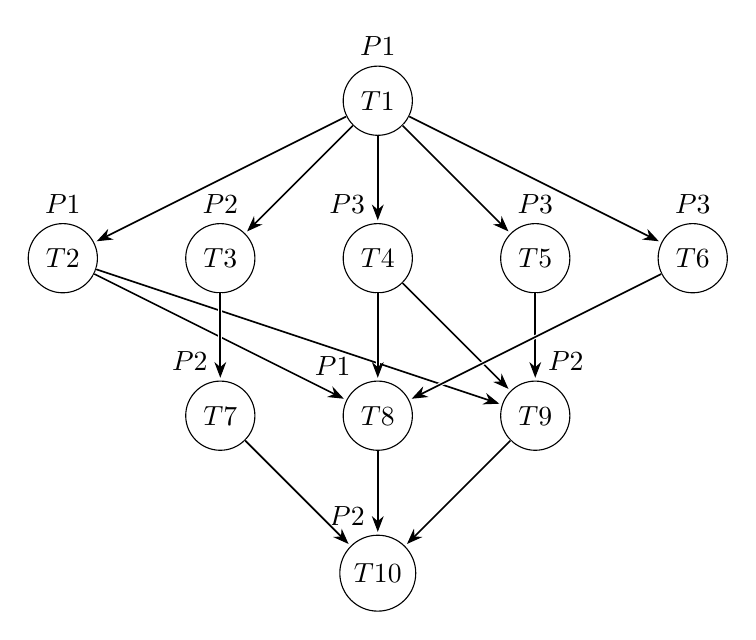
\begin{tikzpicture}[>={Stealth[color=black]},shorten >=1pt,node distance=2cm,on grid,initial/.style={}]
        \node[state, label=above:$P1$] (T1) {$T1$};
        \node[state, label=95:$P3$] (T4) [below =of T1] {$T4$};
        \node[state, label=above:$P2$] (T3) [left  =of T4] {$T3$};
        \node[state, label=above:$P1$] (T2) [left  =of T3] {$T2$};
        \node[state, label=above:$P3$] (T5) [right =of T4] {$T5$};
        \node[state, label=above:$P3$] (T6) [right =of T5] {$T6$};
        \node[state, label=120:$P1$] (T8) [below =of T4] {$T8$};
        \node[state, label=95:$P2$] (T7) [left  =of T8] {$T7$};
        \node[state, label=85:$P2$] (T9) [right =of T8] {$T9$};
        \node[state, label=95:$P2$] (T10) [below =of T8] {$T10$};
        \begin{scope}[every edge/.append style={->, double=black, draw=white}]
          \path (T1)
            edge   (T2)
            edge   (T3)
            edge   (T4)
            edge   (T5)
            edge   (T6);
          \path (T2)
            edge   (T8)
            edge   (T9);
          \path (T3) edge   (T7);
          \path (T4) edge   (T8);
          \path (T4) edge   (T9);
          \path (T5) edge   (T9);
          \path (T6) edge   (T8);
          \path (T7) edge   (T10);
          \path (T8) edge   (T10);
          \path (T9) edge   (T10);
        \end{scope}
      \end{tikzpicture}
  }
  \caption{Market Access}
  \label{fig:f2}
\end{figure}


% == END
\end{document}